% Preamble
\documentclass[12pt]{article}

% Packages
\usepackage{amsmath}
\usepackage{hyperref}
\usepackage[utf8]{inputenc}
\usepackage[T1]{fontenc}
\usepackage{graphicx}
\usepackage{color}
\usepackage{rotating}
\usepackage{float}

\title{\textbf{Zufallszahlen Spektraltest}}
\author{Christian Locatelli, Alexander Wallrodt}
\date{\today}

% Document
\begin{document}
    % Titelseite
    \maketitle
    \clearpage

    % Inhaltsverzeichnis
    \tableofcontents
    % Liste der Tabellen
    \listoftables
    % Liste der Bilder
    \listoffigures

    \clearpage

    \section{Einleitung}\label{sec:Einleitung}
    Im folgenden Projekt geht es um die Frage, inwieweit von einem Computer per Algorithmus erzeugte Pseudo-Zufallszahlen
    auch wirklich als zufällig zu Erachten sind.
    Es werden daher insgesamt vier unterschiedliche Zufallszahlengeneratoren mit einem Sprektraltest untersucht und dabei erörtert,
    ob zwischen den erzeugten Zufallszahlen ein kausaler Zusammenhang besteht,
    oder ob diese Generatoren den Zufall gut simulieren können.



    \section{Das Pythonscript}\label{sec:das-pythonscript}
    Wie ist das Pythonscript aufgebaut und wie funktioniert es?

    \subsection{Der LCG}\label{subsec:der-lcg}
    Der LCG ist ein einfacher Generator, welcher mit den Startwerten $a$, $x_n$, $c$, $m$ aufgerufen wird.
    $a$ ist der Faktor, $n$ der Startwert, $c$ ist das Inkrement und $m$ der Modulus.
    Diese können beliebig gewählt werden, jedoch nur bestimmte sehen auch zufällig aus.
    Für unser Projekt haben wir die Werte des TI-59 von Texas Instruments gewählt~\cite{lcg}.

    \begin{align*}
    x_n = (a * x_n + c) \bmod m
    \end{align*}

    \subsection{Der Random.org Generator}\label{subsec:der-random.org-generator}
    Random.org ist eine Internetseite, die sich darauf spezialisiert hat, Zufallszahlen zu erzeugen.
    Sie wird unter anderem für Lotterien und Online-Spiele, aber auch für diverse wissenschaftliche
    Anwendungen verwendet.
    Hierbei behaupten die Entwickler, der Generator würde mithilfe von atmosphärischem
    Rauschen echte Zufallszahlen erstellen, die besser sind als die von Computer erstellten Pseudo-Zufallszahlen~\cite{random-org}.

    \subsection{Die Zufallsgeneratoren von Python}\label{subsec:die-zufallsgeneratoren-von-python}
    Python hat selbst verschiedene Zufallszahlengeneratoren integriert, die Pseudo-Zufallszahlen erstellen können.
    Hierbei wird der sogenannte Mersenne-Twister verwendet, welcher floats in einer Genauigkeit von 53 Bit erzeugt und welcher
    eine Periode von $p=2^{19937}-1$ besitzt.
    Er gilt als einer der am häufigsten getesteten Zufallsgeneratoren, ist jedoch vollständig deterministisch,
    weswegen er beispielsweise für Kryptografie ungeeignet wäre~\cite{python-random,mersenne-twister}.
    Im Programm werden die Methodem \texttt{random.random()} und \texttt{numpy.random.random()} getestet,
    welche eine Fließkommazahl zwischen 0 und 1 erzeugen.



    \section{Ergebnisse}\label{sec:Ergebnisse}
    Um die Generatoren auf ihre Zufälligkeit zu überprüfen wurde der Spektraltest verwendet.
    Bei diesem werden Tupel gebildet, welche man als Punkt im dreidimensionalen Raum interpretiert und darstelllt.
    Ziel ist dabei eine gleichmäßig verteilte Menge von Tupeln.
    Wenn sich jedoch Muster erkennen lassen kann man direkt festhalten, dass ein stochastische Abhängigkeit vorherrscht~\cite{spektraltest}.
    In diesem Projekt wurden zur Veranschaulichung 2er-Tupel und 3er-Tupel gebildet,
    welche in einem XY-Diagramm beziehungsweise XYZ-Diagramm dargestellt sind.
    Der Spektraltest wurde dabei auf jeden der vier verschiedene Generatoren angewandt.
    Um einen guten Vergleich der Generatoren zu ermöglichen, geben alle Generatoren Fließkommazahlen zwischen 0 und 1 zurück.
    Bei jedem Generator wurden 100.000 Zufallszahlen abgerufen, jedoch ist man bei Random.org beschränkt,
    weswegen dort nur 10.000 Zufallszahlen abgerufen wurden.

    \begin{table}

        \caption[Ergebnisstabelle]{Ergebnisstabelle}

        \centering

        \begin{tabular}{|c||c|c|}

            \hline
            & XY-Tupel & XYZ-Tupel \\


            \hline
            \hline
            \rotatebox{90}{LCG} &
            \begin{figure}
                \centering
                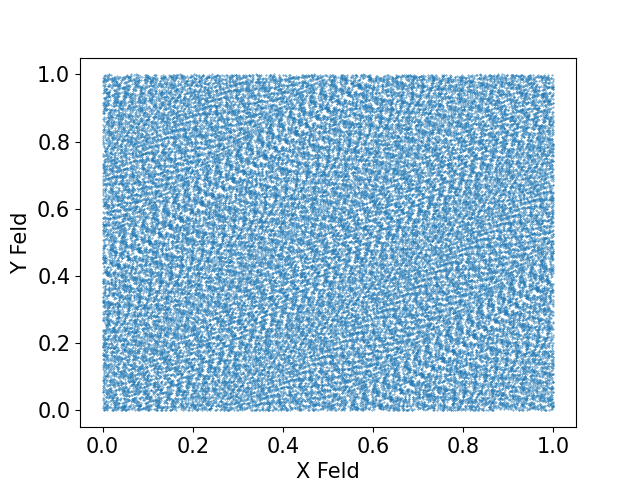
\includegraphics[width=6cm]{images/Random_numbers_by_lcg_with_an_amount_of_100000_numbers_in_2D}
                \caption[LCG Generator mit 100000 Zahlen in 2D]{LCG Generator mit 100000 Zahlen in 2D}
                \label{fig:figure}
            \end{figure}

            &
            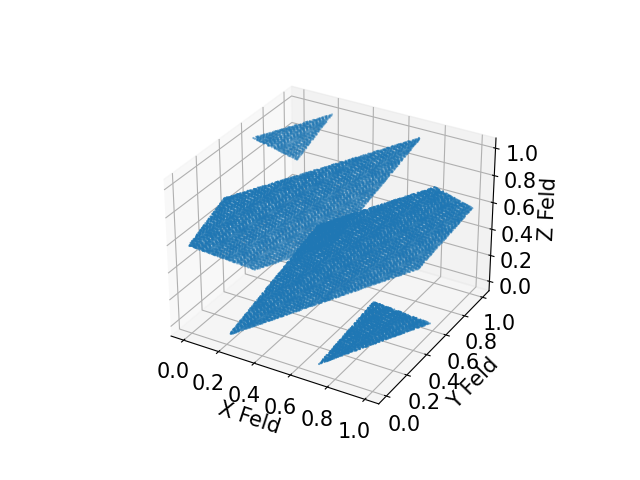
\includegraphics[width=6cm]{images/Random_numbers_by_lcg_with_an_amount_of_100000_numbers_in_3D} \\

            \hline
            \rotatebox{90}{Random Library} &
            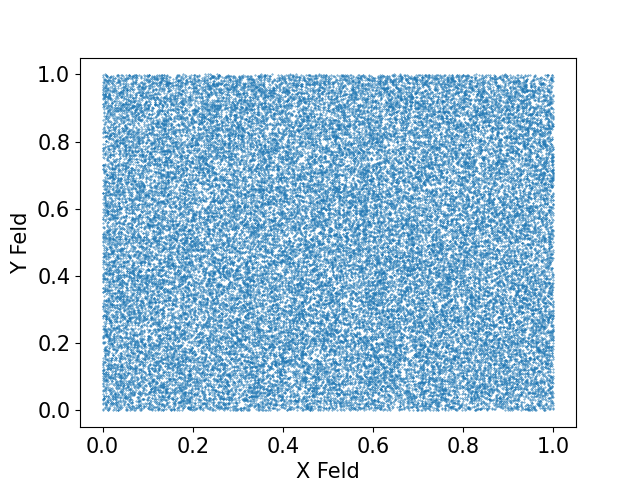
\includegraphics[width=6cm]{images/Random_numbers_by_random_lib_with_an_amount_of_100000_numbers_in_2D} &
            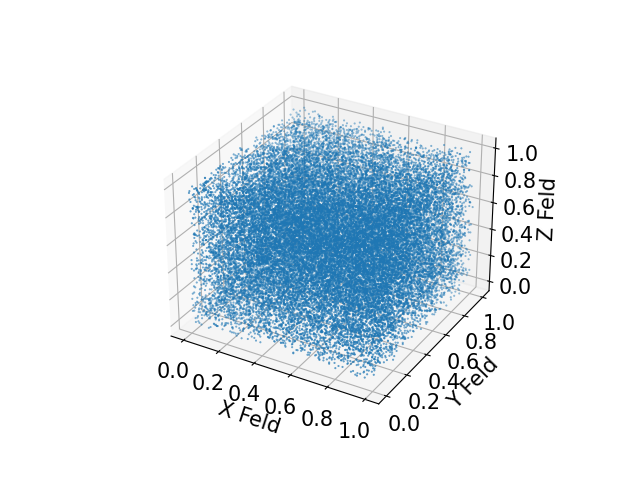
\includegraphics[width=6cm]{images/Random_numbers_by_random_lib_with_an_amount_of_100000_numbers_in_3D} \\

            \hline
            \rotatebox{90}{Numpy Library} &
            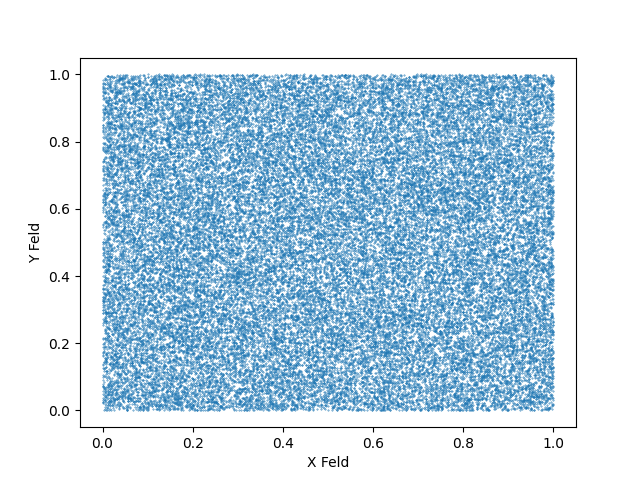
\includegraphics[width=6cm]{images/Random_numbers_by_numpy_lib_with_an_amount_of_100000_numbers_in_2D} &
            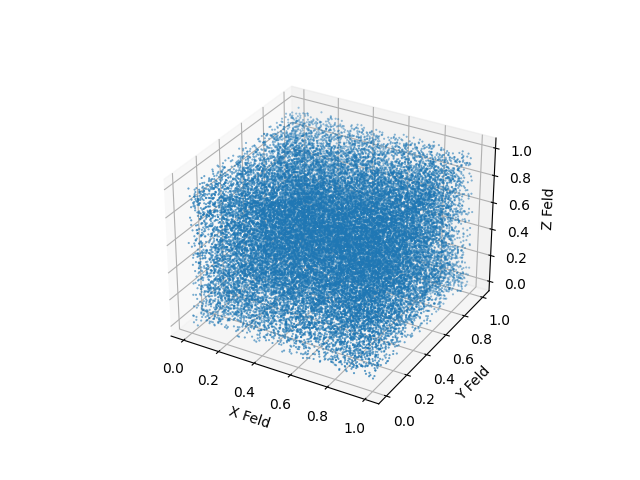
\includegraphics[width=6cm]{images/Random_numbers_by_numpy_lib_with_an_amount_of_100000_numbers_in_3D} \\

            \hline
            \rotatebox{90}{Random.org} &
            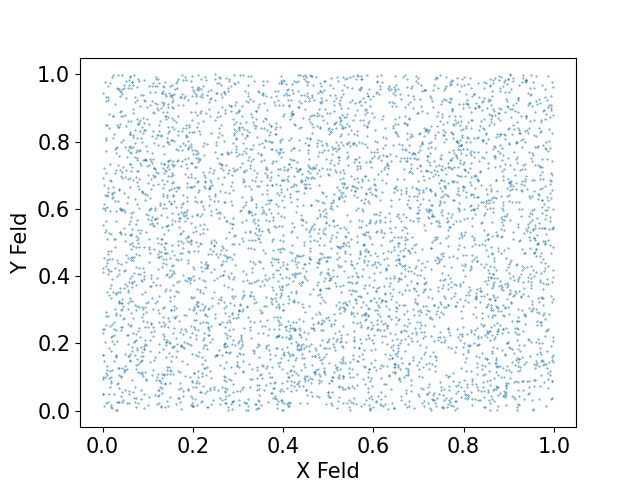
\includegraphics[width=6cm]{images/Random_numbers_by_random_org_with_an_amount_of_10000_numbers_in_2D} &
            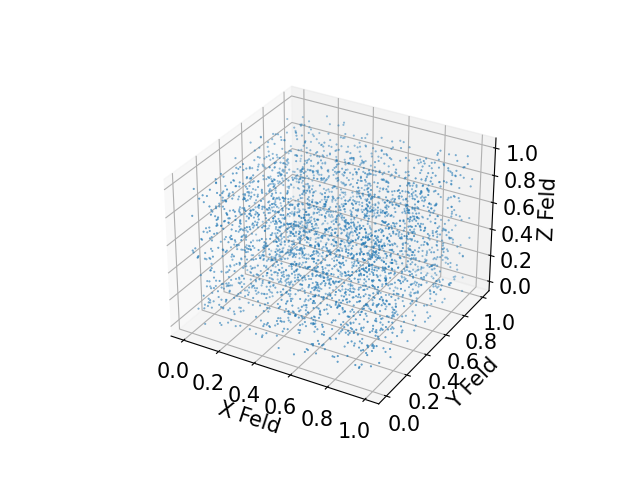
\includegraphics[width=6cm]{images/Random_numbers_by_random_org_with_an_amount_of_10000_numbers_in_3D} \\

            \hline

        \end{tabular}\label{tab:ergebnisse}

    \end{table}

    \subsection{Fazit}\label{subsec:fazit}
    Die Ergebnisse zeigen, dass der LCG kein guter Generator ist, da in der 3D- und 2D-Darstellung Muster zu erkennen sind und somit ein kausaler Zusammenhang zwischen den erzeugten Tupeln besteht.
    Die Tupel in den Zufallsgeneratoren der Python-Bibliotheken sind dagegen sehr gleichmäßig verteilt.
    Man könnte daher schlussfolgern, dass es sich um zufällig erstellte Zahlen handelt.
    Da die Bibliotheken jedoch wie beschrieben auf dem Mersenne-Twister basieren, bei welchem man erst ab einer sehr hohen Periode Kausalitäten erkennen würde,
    können die Generatoren lediglich als "gute" Pseudozufallszahlengeneratoren bezeichnet werden.
    Die Tupel vom Generator der Seite Random.org sind ebenfalls sehr gleichmäßig verteilt und es lassen sich keine Muster erkennen.
    Man bräuchte allerdings eine viel größere Menge von Zufallszahlen, um zu beweisen, dass der Generator "echte" Zufallszahlen erzeugt.
    Durch die Angaben der Entwickler lässt sich aber zusammenfassend festhalten, dass dies der beste Generator ist.


    \vfill

    \begin{thebibliography}{12345}

        \bibitem{lcg}
        \url{https://de.wikipedia.org/wiki/Kongruenzgenerator}

        \bibitem{random-org}
        \url{https://www.random.org/analysis}

        \bibitem{random-org-api}
        \url{https://www.random.org/clients/http/}

        \bibitem{python-random}
        \url{https://docs.python.org/3/library/random.html}

        \bibitem{mersenne-twister}
        \url{https://de.wikipedia.org/wiki/Mersenne-Twister}

        \bibitem{spektraltest}
        \url{https://de.wikipedia.org/wiki/Spektraltest}

    \end{thebibliography}

\end{document}